\chapter{Identity and authentication on the Web}
\label{ch:identity}
Digital identity credentials such as passwords, tokens and keys are used to ensure that only authorized users are able to access online services. Because such services manage sensitive and valuable information, they have become attractive targets for a variety of online attacks. For example, online financial services must use stronger credentials for authentication to avoid fraud. Because of serious threats and widespread theft and misuse of identity credentials, there is considerable interest in the area of identity management, which addresses secure use of identity credentials.\\

Decentralized, user-centric identity management offers better privacy and control over the use of identity credentials, since it allows users to flexibly choose what identity information is released to other entities in each transaction. For instance, users may choose to use a trusted identity provider (IdP) that they believe is the most appropriate for each transaction, or they may even use their own identity provider, therefore allowing them to control what identity information is disclosed to service providers (SP).\\

In this context, we propose an identity management system architecture based on the concept of decentralized identity provider, which coupled with an efficient access control system, ensures that identity credentials remain under the user's control.\\

This chapter is structured as follows. Section~\ref{sec:identity_sota} provides an overview of existing solutions. Section~\ref{sec:webid} presents our first contribution, Web Identity and Discovery (WebID), followed by a privacy and security analysis. Section~\ref{sec:webid-auth} presents our second contribution, the WebID-TLS authentication protocol. Section~\ref{sec:webid-delegated-access} discusses the possibility of using a third-party authentication service in cases where Web applications cannot directly implement the WebID-TLS protocol. Section~\ref{sec:webid-delegated-access} covers the topic of delegating an agent to act on behalf of a user in order to no longer require the user's presence when making authenticated requests. Finally, we compile and present a list of conclusions.

\section{Related work}
\label{sec:identity_sota}
In this section, we start by reviewing related work in user-centric identity management area, while discussing the issues and threats against existing user-centric identity management schemes. We decided to investigate the protocols which provide users with identity, authentication and attribute exchange (i.e. providing additional data about the user), while ignoring the protocols that focus on one specific aspect.\\

The identity and authentication protocols that we will present next are based on three common entities. The first one is the user, or more commonly the browser, which is typically responsible for authentication. Next is the service provider (SP), which is usually a Web application. Finally, we have the identity provider (IdP), which also acts as an attribute provider, and whose task is to handle requests for the user's identity data.


\subsection{OpenID Connect}
\label{subsec:openid}
OpenID~\cite{recordon2006openid} is a lightweight identity management system originally designed for relatively simple applications, such as blog services. While the OpenID brand has undergone several major changes, its latest iteration called OpenID Connect~\cite{sakimura2011openid} is a profile of OAuth~2.0~\cite{hammer2011oauth}, optimizing certain elements of OAuth for server-side exchange of attributes while requiring no changes to current browsers. OAuth is a standard for granting data authorization to third parties, allowing people to grant access to private resources after authenticating themselves via their online identity. OpenID Connect uses OAuth 2.0 for the authorization flow, though it adds a small number of attributes in the response between an identity provider and the service provider. One important point is that OpenID Connect, as it is a profile of OAuth, does not standardize any authentication, but only specifies an HTTP redirection flow from the service provider to the identity provider. In current implementations of OpenID, authentication is usually done via a user name and password combination.\\

\begin{figure}[htbp]
  \begin{center}
    \includegraphics[width=200px]{img/openid.pdf}
        \caption{Flow of OpenID Connect (based on OAuth 2.0).}
        \label{fig:openid-flow}
  \end{center}
\end{figure}

Figure~\ref{fig:openid-flow} depicts the necessary steps that have to be taken in order to successfully permit to a service provider to access a user's personal attributes.

\begin{enumerate}
\item A user visits a service provider (SP) that needs attributes.
\item The SP makes a request for attributes to the identity provider (IdP).
\item The user is redirected to the IdP from the SP.
\item The user authenticates to the IdP (typically using a username-password combination), and is granted a bearer token.
\item The user is redirected back to the SP and grants an authorization token to the SP.
\item The SP sends the authorization token to the IdP and receives an access token (a bearer token with a specific scope and a limited lifespan).
\item While the access token is valid, the IdP sends attributes to the SP.
\end{enumerate}

Authentication is out of scope of OpenID Connect specification, but the flow usually relies on redirects and it is by default based on usernames and passwords. Authorization relies on OAuth 2.0 and a server-side flow is fully specified that works even when the user is offline, once the user has granted authorization. This is a distinct advantage for use-cases involving aggregation and inter-application communications. Therefore, we can consider that OpenID Connect offers an "offline client; server-to-server" authorization flow.\\

Redirection attacks are possible with OpenID Connect. Unless the user is aware that TLS is enabled, a malicious service provider can fool them into redirecting to a fake identity provider site and then use that redirection to intercept their real credentials (i.e. usually passwords). The malicious party can then reuse the stolen credentials to provide a real authorization code to the actual identity provider, effectively impersonating the real user. There are a number of variations on this attack, such as a real identity provider being provided with a malicious redirection URI to fake a valid service provider.\\

Even though validity lifespans, one-time authorization codes and tokens provide increased security, a bearer token can be intercepted and used in an attack. This is possible because bearer tokens are authorization credentials which are later used in OpenID, once authentication has been performed. As all authorization credentials are transmitted via HTTP user-agent redirections, these credentials can be revealed possibly via HTTP referrer headers and the browser history. Additionally, once an access token is granted, the service provider can talk to the identity provider without any interaction with the user. The user does not necessarily know the scope, lifetime, and kinds of access to their attributes that a token provides. Furthermore, the identity provider can observe every interaction of the user with any service provider.

\subsection{Mozilla Persona}
Mozilla Persona~\cite{browserid} (formally known as BrowserID) allows users to authenticate by proving their identity via a \textit{verified} email address, and demonstrates the user's ownership of the addresses to service providers using a cryptographic proof. Unlike OpenID Connect which requires trust in the server, Persona requires trust in the browser. The system allows an identity provider to store a secure, revocable key representing a user authentication into a browser. It also indicates to the browser the terms of use of the key, so that it can be expired, invalidated, and refreshed as needed. With some additional work, it can be used to create pseudonymous identities that allow a user to provide a different address per service provider.\\

\begin{figure}[htbp]
  \begin{center}
    \includegraphics[width=200px]{img/browserid.pdf}
        \caption{Flow of Mozilla Persona.}
        \label{fig:browserid-flow}
  \end{center}
\end{figure}

Figure~\ref{fig:browserid-flow} depicts the necessary steps to successfully authenticate using Mozilla Persona.

\begin{enumerate}
\item The user attempts to identify himself/herself by providing an e-mail address, in order to bind that address to a particular set of cryptographic keys (for which the user then provides a proof of possession) by having the IdP attest to that binding.
\item The browser checks to see if a private key associated with that email address is present in the browser.
\item If no key exists in the browser for that specific email address, then the browser generates key material and registers the public key with the IdP.
\item The browser sends a signed authentication credential to the SP.
\item The SP verifies the authentication credentials with their locally stored database of IdP public keys, authenticates the user if verification succeeds (not shown in diagram as this step does not happen with every transaction).
\item The browser sends signed attributes to the SP.
\end{enumerate}

As authentication is done by default using cryptographic keys as opposed to username-passwords, it is much more secure. Furthermore, there is no need for redirection. This specification does not explicitly set parameters for the authorization scope, but it enables a browser-mediated flow of verified attributes. The drawback is that it only works if the browser is online.\\

Although the service provider knows the identity provider's key and will have to check at least once with the identity provider to determine public key of user, it does not have to check in theory more than once per e-mail (although updates should be done at set time intervals though less frequently than user transactions). It must be noted that using email address as identifiers enables the linking of transactions. However, email addresses can be short-lived or they can be used as pseudonymous.\\

Unfortunately, all verification of cryptographic keys from the browser is done by a centralized service (http://www.browserid.org),
which would be a major vulnerability if compromised. Ironically, the registration to the IdP such as http://www.browserid.org is currently done with user names and passwords.\\

In the end, the Mozilla Persona operation model could simply be considered proof of a \textit{login and check email} capability, similar to other systems which rely on emails to reset forgotten passwords. Therefore, the security of the system relies on the security of the IdP - in this case the email provider. Given the poor state of the security for many email providers (e.g. STARTLS not providing warning messages if TLS does not work, allowing e-mails to be transmitted as cleartext), the possibility of email address compromise greatly affects this system. 

\subsection{Web Authentication}
A recent effort comes in the form of Web Authentication~\cite{dahl2013web}, a JavaScript-based cryptographic library standardized by the W3C Web Cryptography Working Group. Web Authentication allows both OpenID Connect and Mozilla Persona authorization flows to take place, while at the same time avoiding the dangerous redirections used by OpenID Connect by replacing the bearer tokens with signed tokens. The main advantage of combining OpenID Connect and Mozilla Persona is that user attributes can be transmitted offline, thanks to OpenID Connect's "offline client; server-to-server" flow, while at the same time offering increased privacy for user attributes thanks to Mozilla Persona's "online client-to-server" flow.

\begin{figure}[htbp]
  \begin{center}
    \includegraphics[width=200px]{img/webcrypto.pdf}
        \caption{Flow of Web Authentication.}
        \label{fig:webcrypto-flow}
  \end{center}
\end{figure}

Figure~\ref{fig:webcrypto-flow} presents the combined flows of OpenID Connect and Mozilla Persona when using Web Authentication.\\

\begin{enumerate}
\item User visits the SP and presents the authentication credential, signed by the IdP.
\item If the user wishes to enable offline attribute access, then the user must register its public key with the IdP and enable that flow.
\item The IdP signs the user's authentication credential and any attributes to be transmitted via the browser.
\item The SP verifies the signature of the authentication credential.
\item If the signature on authentication credential is valid, then the user is authenticated and verified attributes can be sent via the browser if needed.
\item In the case of authorized offline flow, signed attributes are sent from the IdP to the SP.
\end{enumerate}

This sort of approach can offer identifiers that are short-lived (or pseudonymous) while maintaining the privacy for user attributes. We can consider email verification to be one of many possible authentication methods, though it is possible to transfer only signed identifiers to the relying party in cases where another form of high-security (i.e. a smartcard) authentication is needed. However, even this system would be vulnerable to traffic analysis, though it can be ameliorated through the use of proxies  and messages being sent regularly and padded.


\subsection{SAML}
The OASIS Security Assertion Markup Language (SAML)~\cite{hallam2001security} standard defines an XML-based framework for describing and exchanging security information between online business partners, and which attempts to tackle the single-sign on (SSO) problem amongst many others. This security information is expressed in the form of portable SAML assertions that applications working across security domain boundaries can trust. Examples of SAML deployment include universities, Google, and Cisco. Unlike many other identity technologies, SAML is able to provide security solutions for banking and government Web portals. SAML is, however, often viewed as being more complex than is necessary to support implementations requiring low levels of assurance. This has driven many developers to deploy simpler technologies like OpenID in low assurance scenarios.\\

In the latest version, SAML 2.0~\cite{cantor2005saml}, the primary use case is still Web Browser SSO, but the scope of SAML 2.0 is broader than previous versions of SAML. The user first authenticates to the identity provider. The user is then able to access a resource at one or more service providers without needing to log in at each service provider. The diagram in Figure~\ref{fig:saml-flow} shows the process for what is known as Service Provider Initiated Single Sign-on, which is what happens when the user visits the service first, and needs to be authenticated.

\begin{figure}[htbp]
  \begin{center}
    \includegraphics[width=300px]{img/saml.pdf}
        \caption{Simple deployment of the SAML 2.0 Web Browser SSO profile, using the HTTP POST binding.}
        \label{fig:saml-flow}
  \end{center}
\end{figure}

\begin{enumerate}
\item The user makes a request to the SP for a specific resource. This request may happen in a variety of ways for a variety of reasons. For example, the user may be following a bookmark or clicking on a link from an email.
\item To begin the authentication process, the SP responds with a document containing an XHTML form, signs it, optionally encrypts it, and encodes it. An organization-specific host name allows the user's organization to be discovered. Along with the SAML Request, an HTTP parameter called \textit{RelayState} is passed along to the IdP. This captures the location of the resource the user originally requested.
\item The user agent issues a POST request to the SSO service at the IdP. The SSO service processes the \textit{AuthnRequest} element (by URL-decoding, base64-decoding and inflating the request, in that order) and performs a security check. If the user does not have a valid security context (i.e. an existing session), the identity provider identifies the user.
\item The SSO service on the IdP validates the request, builds the \textit{SAMLResponse} and responds with a document containing an XHTML form. The value of the \textit{RelayState} parameter has been preserved from Step 3.
\item The user (browser) issues a POST request to the assertion consumer service at the SP, where the values of the \textit{SAMLResponse} and \textit{RelayState} parameters are taken from the XHTML form at Step 4.
\item The assertion consumer service processes the response, creates a security context (i.e. a session) to log the user into the SP and redirects the user to the requested resource.
\end{enumerate}

SAML does not specify the method of authentication at the identity provider; it may use a username/password, multifactor authentication, etc.. A directory service, which allows users to login with a user name and password, is a typical source of authentication tokens (i.e. passwords) at an identity provider. Any of the popular common internet social services also provide identity services that in theory could be used to support SAML exchanges.\\

Since it is XML-based, SAML has extensibility, which makes it a very flexible standard. Two federation partners can choose to share whatever identity attributes they want in a SAML assertion (message) payload as long as those attributes can be represented in XML. Interoperability also gives SAML a huge advantage over proprietary SSO mechanisms, which require the identity provider and SP to both implement the same software. Additionally, a single SAML implementation can support SSO connections with many different federation partners.\\

SAML was designed to be robust when it comes to security threats as well as user data privacy. However, an in-depth description of possible attack scenarios and countermeasures has been provided by OASIS in~\cite{maler2005security}.\\


\subsection{Synthesis}
Unfortunately, neither of the aforementioned protocols offer true decentralization, since service providers offer a limited number of choices for identity providers, based on a priori trust relationships between them. Additionally, even though some user attributes are transmitted once authentication has been performed, the user is usually forced to create a local account on the new service provider, thus moving from one silo to another. Moreover, username and passwords are still the preferred choice when it comes to authentication credentials, decreasing the security of the system.\\

In the next section we will present the first of our contributions, a decentralized, user-centric identity scheme based on the Semantic Web, which hopes to address existing issues present in popular decentralized authentication protocols.


% WebID
\section{Web Identity and Discovery - WebID}
\label{sec:webid}
A global distributed Social Web requires that each person be able to control their identity and that this identity be linkable across sites, thus placing each person in a Web of relationships.\\

WebID~\cite{webid2013}, our first contribution, is a simple and universal identification mechanism that is distributed, openly extensible, improves privacy, security and control over how each person can identify themselves. It does this by applying the best practices of Web Architecture whilst building on well established widely deployed protocols and standards including HTML~\cite{berners1995hypertext}, URIs~\cite{berners1998uniform}, HTTP~\cite{berners1996hypertext}, and RDF semantics. WebID is a work-in-progress open standard within the World Wide Web Consortium\footnote{http://w3.org}, to which we are actively contributing.\\

The general idea behind WebID is that Agents (e.g. a person, an organization, a group, etc.) create their own identities by linking a \textit{unique identifier} (i.e. an HTTP URI) to a \textit{profile document}, a type of Web page that any Web user is familiar with, and which uses a standardized RDF serialization format. The profile document contains all the necessary information to create a Web of trust which allows people to link together their profiles in a public or protected manner. Such a Web of trust can then be used by Web services to make authorization decisions, by allowing access to resource depending on the properties of an agent, such that he/she is known by some relevant people, works at a given company, is a family member, is part of some group, etc..\\

Before explaining how WebID works, we must provide definitions for several terms we have used or we will be using.\\

\textbf{Server} - a device contactable at a domain name or IP address that hosts a number of globally accessible services.\\

\textbf{Service} - an application or agent listening for requests at a given IP address and port number on a given server.\\

\textbf{Requesting Agent} - an agent that initiates a request to a service, on a given server.\\

\textbf{WebID} - a URI with an HTTP or HTTPS scheme which denotes an Agent (Person, Organization, Group, Device, etc.).\\

\textbf{WebID Profile} - an RDF document which uniquely describes the Agent denoted by the WebID in relation to that WebID.\\

\textbf{Dereferencing a URI} - in the current context of the Semantic Web, the operation of dereferencing a URI results in accessing the information resource on the Web (located at the given URI) and extracting the RDF semantics from it.\\

\textbf{Hash URI} - a URI containing a fragment identifier (i.e. \#me). The hash symbol (\#) separates the URI to be looked up, the so called \textit{document URI} part of the URI which comes before the \#, from the \textit{relative URI} part which is considered to be an inner reference within the document. When a hash is present, the lookup operation is performed on the document URI.\\

\textbf{Pointed Graph} - a graph that is part of an RDF document and that can be referred to by its relative URI (i.e. <\#me>). The difference between the \textit{named graph}~\cite{carroll2005named} and pointed graph is that the latter is used to refer to a resource that is part of a named graph, and that whose context is only valid within that named graph.\\

To exemplify these terms, Figure~\ref{fig:webid} describes the relations between Tim Berners-Lee's WebID (i.e. the URI) and the profile document to which it refers.\\

The WebID URI - http://www.w3.org/People/Berners-Lee/card\#i - is an \textit{identifier} that refers to a person or more generally an agent, in this case to Tim Berners-Lee.\\

The WebID Profile URI - http://www.w3.org/People/Berners-Lee/card - denotes the \textit{document} describing the agent to which the WebID URI refers. The profile may contain any number of relations describing the agent. For example a user can publish a depiction of himself, so that once authenticated a service can personalize the user experience. The user can also post links to known people, who in turn have WebIDs published on other sites, in order to create a Social Web. More importantly, the user can publish one or more relations to principals used by different authentication protocols. More information on WebID authentication can be found later on in Section~\ref{sec:webid-auth}.

\begin{figure}[htbp]
  \begin{center}
    \includegraphics[width=350px]{img/WebID-overview.png}
        \caption{The relation between the user (Tim Berners-Lee), the WebID URI (http://www.w3.org/People/Berners-Lee/card\#i) and the profile document (http://www.w3.org/People/Berners-Lee/card).}
        \label{fig:webid}
  \end{center}
\end{figure}

\subsection{The WebID URI}
\label{subsec:webid_uri}
On the Semantic Web, URIs identify not just Web documents, but also real-world objects like people and cars, and even abstract ideas and non-existing things like mythical heroes. We can refer to these as real-world objects or things. For example, the person Ann is described on her homepage. Barry may not like the look of the homepage, but may want to link to the person Ann. Therefore, two URIs are needed, one for Ann, one for the homepage or an RDF document describing Ann.\\

In our case, the WebID URI must be one that dereferences to a document the user controls. For example, if a user Barry controls the server hosting https://barry.example/profile, then his WebID URI can be https://barry.example/profile\#me.\\

The main reason why fragment identifiers, commonly known as hashes (i.e. \#me), were introduced is that the WebID URI and the profile document URI should not be the same. If they were the same, then there would be no way to differentiate between the profile document's URI - https://barry.example/profile - and the URI pointing to the profile graph within the document (i.e. \textit{\#me}), which describes the user. In other words, for hash WebIDs, the URI without the hash denotes the \textit{profile document}.\\

However, if hash URIs cannot be utilized, then an HTTP request on the WebID must return an HTTP 303 response with a \textit{Location} header URI referring to the profile document. Hash URIs are encouraged when choosing a WebID since HTTP 303 redirects impact performance for clients by means of additional requests. From here on, all examples will contain such hash URIs.


\subsection{The WebID profile document}
\label{subsec:webid_profile}
Personal details are the most common requirement when registering an account with a website. Some of these pieces of information include an e-mail address, a name and perhaps an image depicting the user. To this regard, WebID profiles are built using vocabularies identified by URIs, that can be placed in subject, predicate or object position of the relations constituting an RDF graph. The definition of each URI is found at the namespace of the URI, by dereferencing it. For example, a \textbf{foaf:name} relation implies that the \textit{foaf:} namespace has been previously defined as a prefix in the following way: \textit{@prefix foaf: <http://xmlns.com/foaf/0.1/>}.\\

The Friend-of-a-Friend (FOAF) vocabulary allows the Semantic Web community to define an open-data social graph. This ontology describes people and their properties, as well as links between people using RDF. In this model, a uniform resource identifier (URI), which in our case is the WebID profile URI, refers to FOAF data representing a person, a group, or their agents and their respective relations. FOAF collects a variety of terms; some describe people, some groups, some documents. Different kinds of applications can use or ignore different parts of FOAF. FOAF descriptions are themselves published as linked documents in the Web (e.g. using RDF/XML, N3, etc.). The result of the FOAF profile is a network of documents describing a network of people and properties. Each FOAF document is itself an encoding of a descriptive network structure.\\

\subsection{Publishing the WebID profile document}
\label{subsec:publishing_webid}
\subsubsection{Content negotiation}
According to W3C guidelines~\cite{jacobs2004architecture}, we have a Web document (also called information resource) if all its essential characteristics can be conveyed in a message (e.g. a Web page, an image or a product catalogue).\\

In HTTP, a 200 response code should be sent when a Web document has been accessed. However, a different Web server configuration is needed when publishing URIs that are meant to identify entities which are not Web documents. Web clients and servers use the HTTP protocol to request representations of Web documents and send back the responses. HTTP has a powerful mechanism for offering different formats and language versions of the same Web document known as \textit{content negotiation}.\\

When a user agent (such as a browser) makes an HTTP request, it sends along some HTTP headers to indicate what data formats and language it prefers. The server then selects the best match from its file system or it may generate the desired content on demand, and then sends it back to the client. For example, a browser could send a specific HTTP request to indicate that it wants a Turtle representation of http://barry.example/people\#me, as seen in Example~\ref{ex:http_request}. We can see that since the client specified that it \textit{Accepts} text/turtle, the server responded with the appropriate \textit{Content-Type}, pointing to the right document.

\begin{example}
\begin{minted}{c}
Request:

GET /people HTTP/1.1
Host: barry.example
Accept: text/turtle


Response:

HTTP/1.1 200 OK
Content-Type: text/turtle
Content-Location: https://barry.example/people
\end{minted}
\caption{Request and response for the Turtle version of the document.}
\label{ex:http_request}
\end{example}

Browsers are also able to announce their ability to consume different formats of RDF, through \textit{Accept} headers that use \textit{q} (quality) values, as seen in Example~\ref{ex:accept_header}.\\

\begin{example}
\begin{minted}{c}
Accept: application/rdf+xml;q=0.7, text/turtle
\end{minted}
\caption{Accept header.}
\label{ex:accept_header}
\end{example}

Here we see that the browser accepts RDF/XML with a q value of 0.7 and Turtle with a q value of 1.0 (the default). This means that the browser has a slight preference for Turtle over RDF/XML, even though the preference for Turtle doesn't necessarily mean that every server should send Turtle. The server has to look at the client's preferences, and then it must make a decision based on the quality of the different variants it could offer.\\

Content negotiation is fairly complex, but in the same time it is a powerful way of choosing the best variant for mixed-mode clients that can deal with HTML and RDF, as well as a decisive factor for interoperability between decentralized Web applications.

\subsubsection{The profile document}
The preferred format for writing WebID profile documents is the Turtle~\cite{beckett2008turtle} notation. The syntax is simple to use and is very similar to the SPARQL~\cite{prud2008sparql} query language, which in turn resembles SQL. Turtle profile documents must be served with the \textit{text/turtle} content type.\\

Take for example the WebID \textit{https://barry.example/profile\#me}, for which the WebID Profile document contains the following Turtle representation, as seen in Example~\ref{ex:webid_profile}.

\begin{example}
\begin{minted}{turtle}
@prefix foaf: <http://xmlns.com/foaf/0.1/> .

<> a foaf:PersonalProfileDocument ;
      foaf:maker <#me> ;
      foaf:primaryTopic <#me> .

<#me> a foaf:Person ; 
      foaf:name "Barry" ; 
      foaf:img <https://barry.example/picture.jpg> ;
      foaf:knows <https://example.edu/p/Ann#MSc> ;
      foaf:knows <https://company.com/p/Sue#i> ;
      foaf:weblog <http://barry.example/blog> .
\end{minted}
\caption{A basic WebID profile document expressed in Turtle.}
\label{ex:webid_profile}
\end{example}

However, a WebID profile document does not need to contain only public resources. A simple way of protecting its contents can be achieved by separating parts of the profile information into separate documents, each protected by access control policies. In the following example, Barry is limiting access to his list of friends, by placing all \textit{foaf:knows} relations into a separate document, as seen in Example~\ref{ex:webid_profile_acl}.

\begin{example}
\begin{minted}{turtle}
@prefix foaf: <http://xmlns.com/foaf/0.1/> .
@prefix rdfs: <http://www.w3.org/2000/01/rdf-schema#> .

<> a foaf:PersonalProfileDocument ;
      foaf:maker <#me> ;
      foaf:primaryTopic <#me> .

<#me> a foaf:Person;
      foaf:name "Barry";
      foaf:img <https://barry.example/picture.jpg> ;
      rdfs:seeAlso <https://barry.example/friends> .
\end{minted}
\caption{The \textit{rdfs:seeAlso} relation is used as reference for the friends section of the profile.}
\label{ex:webid_profile_acl}
\end{example}

In this case, \textit{https://barry.example/friends} is a URI pointing to an ACL protected document containing a list of people known by Barry (cf. Example~\ref{ex:webid_profile_friends}).

\begin{example}
\begin{minted}{turtle}
@prefix foaf: <http://xmlns.com/foaf/0.1/> .

<> a foaf:PersonalProfileDocument;
      foaf:maker <https://barry.example/profile#me>;
      foaf:primaryTopic <https://barry.example/profile#me>.

<https://barry.example/profile#me> a foaf:Person;
      foaf:knows <https://example.edu/p/Ann#MSc> ;
      foaf:knows <https://company.com/p/Sue#i> .
\end{minted}
\caption{The contents of \textit{https://barry.example/friends}.}
\label{ex:webid_profile_friends}
\end{example}


\subsection{Extending the WebID profile document}
\label{subsec:extending_webid}
A notable advantage of WebID over other identity schemes is that WebID can be easily extended. By simply expressing different information through additional vocabularies, WebID profile documents have the useful characteristic that they can be easily merged, allowing partial and decentralized descriptions to be combined in interesting ways. In WebID profile documents, additional vocabularies can be used either to extend the user's personal profile, by means of providing location coordinates, a list of personal interests and more, as well as to describe different activities related to the user - e.g. the user's blog posts, projects to which he/she contributes, etc.

\begin{example}[htbp]
\begin{minted}{turtle}
@prefix foaf: <http://xmlns.com/foaf/0.1/> .
@prefix sioc: <http://rdfs.org/sioc/ns#> .
@prefix   dc: <http://purl.org/dc/terms/> .

<> a foaf:PersonalProfileDocument ;
      foaf:maker <#me> ;
      foaf:primaryTopic <#me> .

<#me> a foaf:Person ; 
      foaf:name "Barry" ;
      foaf:weblog <http://barry.example/blog> .

<http://barry.example/blog/posts/1> a sioc:Post ;
      sioc:has_creator <#me> ;
      dc:title "Hello world!" ;
      sioc:content "This is my first post." .
\end{minted}
\caption{The WebID profile document containing a blog post, expressed using SIOC.}
\label{ex:webid_sioc}
\end{example}

For instance, a WebID profile document can be extended to contain blog posts by using an ontology called the Semantically-Interlinked Online Communities (SIOC)~\cite{breslin2005towards}. From Example~\ref{ex:webid_sioc}, we can easily tell that Barry has a blog post at the URI \textit{http://barry.example/blog/posts/1}, having the title \textit{Hello world!} and a specific content.\\

Additionally, if a user is involved in different projects, he/she can express this through the Description of a Project (DOAP)~\cite{dumbill2012doap} ontology. In Example~\ref{ex:webid_doap}, Barry states that he is a developer for a project called \textit{My Project}. By expressing this fact through linked data, any service is now able to dereference the URI for the project - i.e. \textit{http://myproject.org/} - in order to discover more information.\\

As you can see, reusing existing vocabularies greatly increases interoperability, since any Semantic Web service will be able to understand the meaning of the data found within a WebID profile document.

\begin{example}
\begin{minted}{turtle}
@prefix foaf: <http://xmlns.com/foaf/0.1/> .
@prefix doap: <http://usefulinc.com/doap/> .

<> a foaf:PersonalProfileDocument ;
      foaf:maker <#me> ;
      foaf:primaryTopic <#me> .

<#me> a foaf:Person ; 
      foaf:name "Barry" .

<http://myproject.org/> a doap:Project ;
      doap:name "My Project" ;
      doap:developer <#me> .
\end{minted}
\caption{The WebID profile document extended with DOAP information.}
\label{ex:webid_doap}
\end{example}


\subsection{Privacy and security analysis}
\label{subsec:webid_limitations}

\subsubsection{Privacy}
As you might have noticed, WebID in its simplest form suffers from the same limitations that affect most persistent identity schemes. Among those limitations, the primary concern is that user privacy can be undermined by tracking/fingerprinting the user across different services. Even though access to all profile information can be restricted through access control policies, by aggregating user data from multiple services, attackers could in theory be able to build a complete profile of the user. Of course, the same hypothesis remains valid for services operated by the same company.\\

A possible solution is to use multiple identifiers (WebID URIs) linked to the same profile document. Short-lived identifiers offer even better protection, though managing them becomes increasingly difficult, especially for users editing their profile documents by hand. Another solution is to investigate a mechanism similar to \textit{Do Not Track} (DNT)~\cite{mayer2011not}, which is a universal third-party Web tracking opt out, but which would enforce access control on external services too.

\subsubsection{Security}
Not using HTTPS when serving the WebID profile document opens the door to man-in-the-middle attacks. This can be currently avoided in two ways. The first way is to host WebID profile document on HTTPS-enabled Web servers. However, relying on HTTPS also implies having to validate the server's certificates through a standard Public Key Infrastructure (PKI) trust chain, which is fundamentally vulnerable because CAs can be compromised and used to replace valid certificates for millions of domains.\\

Alternatively, the new DNS-Based Authentication of Named Entities (DANE)~\cite{hoffman2012dns} protocol offers the option to use the DNSSEC~\cite{ateniese2001new} infrastructure to store and sign keys and certificates that are used by TLS. DANE is envisioned as a preferable basis for binding public keys to Domain Name System (DNS) names, because the entities that vouch for the binding of public key data to DNS names are the same entities responsible for managing the DNS names in question. In other words, DANE allows the site owners to publish their certificates in DNS.\\

In the next section we will present an authentication protocol based on WebID and client certificates in Web browsers, which does not rely on the classic PKI infrastructure in order to build trust.


\section{WebID-TLS}
\label{sec:webid-auth}
The classic means of authentication are the use of \textit{something you know} (i.e. a password), \textit{something you have} (i.e. a hardware token), or \textit{something you are} (i.e. a fingerprint). While this can encompass cryptographically generated one-time passwords~\cite{haller1996one}, sophisticated smart cards~\cite{schnorr1990efficient} or biometrics~\cite{snelick2005large}, these technologies are expensive to deploy and even more expensive to manage efficiently. Most Web sites use the now-familiar password, something that is known only to the user and the web service.\\

Passwords place the smallest initial burden on both parties in order to form a trusted relationship. They are, however, a serious weak link in the chain of trust, as users have been shown to be bad at devising passwords that are robust against guessing. To make things worse, passwords are reused across domains and applications, so that if one web server has been compromised, an attacker may potentially take advantage of an entity's identity across multiple sites.\\

Passwords serve as a basis of trust, but they require an infrastructure for delegation and transfer of trust. The most basic model of trust is simply the user trusting the website. This classic model reflects the human model of trust, but does not work for the complex online world, where much of the transaction is hidden~\cite{camp2007reliable}. Between the user and the service provider lie a number of technical and organizational layers: the browser, the Internet Service Provider (ISP), and the standards and systems ensuring interoperability. These layers have different models of trust, some stronger than others. The certificate management system used to trust digital certificates for the secure exchange of information via SSL/TLS uses a monolithic system of trust through association. There exists a large set of Certification Authorities (CAs) from whom a web site can obtain a certificate used for these secure transactions. The web browser will automatically only engage in a secure connection with a web browser if the Web site's certificate is approved by the one of the established set of CAs. There exists, however, a key flaw in this trust model. Users have no way of differentiating between CAs, and there is increasing evidence that some are not trustworthy at all~\cite{arnbak2012certificate}.\\

\subsection{Introduction}
\label{subsec:webid-tls_idea}
Our second contribution, the WebID-TLS authentication protocol~\cite{webid-tls}, enables secure, efficient and user friendly authentication on the Web by allowing people to choose a client certificate proposed to them by their browser during the authentication process. A very important aspect of WebID-TLS is that it replaces standard username-password authentication methods, At the same time, it is easy to implement since it takes advantage of the cryptography behind the Transport Layer Security (TLS) protocol~\cite{dierks2008transport}. Furthermore, it is not affected by the same issues that are common to PKIs, since it does not rely on Certification Authorities. Using self-signed certificates also means reducing costs created from issuing certificates by trusted CAs.\\

The main advantage of WebID-TLS is the fact that it is a truly decentralized authentication protocol, with no pre-existing trust relationships required between the SP and the IdP, unlike the authentication protocols presented in Section~\ref{sec:identity_sota}. In WebID-TLS, trust is built by using the Semantic Web to imaginatively reason over the contents of the profile document. For example, a user can be granted access to a protected resource because the owner of the resource has an access control rule stating: "give \textit{read} access to all users with whom I share a minimum of X friends". Another rule would allow access to users having a WebID hosted on a domain that has been previously white-listed. It is up to each service provider to decide on the granularity on which it grants access to users.

\subsection{WebID-TLS terminology}
\label{subsec:webid-tls_terms}
Building on the WebID concepts presented above, several new terms must now be defined.\\

\textbf{Certificate} - is a cryptographic document binding a public key to a user/agent's distinguished name (DN), or in the case of WebID-TLS, to the \textit{SubjectAlternativeName}.\\

\textbf{WebID Certificate} - is a standard X.509 certificate~\cite{solo1999internet} that is used to identify an Agent using one or more WebIDs. The certificate does not need to be signed by a well known CA. However, it can be signed by a trusted CA, by the server which hosts the WebID Profile, or it can even be self signed. The certificate must contain a \textit{SubjectAlternativeName} extension with at least one WebID URI entry identifying the user/agent. Dereferencing this URI should return a representation containing RDF data.  A typical SAN extension value for a certificate identifying the WebID \textit{https://barry.example/profile\#me} can be observed in Example~\ref{ex:webid_cert}.\\

\begin{example}
\begin{minted}{c}
X.509v3 extensions:
      ...
      X509v3 Subject Alternative Name:
            URI:https://barry.example/profile#me
\end{minted}
\caption{The Subject Alternative Name extension of an X.509 certificate.}
\label{ex:webid_cert}
\end{example}

\textbf{TLS Service} - secures the transport layer before passing messages to the application layer service itself (in this case the HTTP server). The TLS protocol~\cite{dierks2008transport} is applied to incoming connections. It identifies the server to the client, securing the channel and is able to request authentication credentials from the client if needed. Server credentials and client credentials traditionally take the form of X.509 certificates containing cryptographic keys. The TLS protocol enables the TLS service to verify that the client controls the private key corresponding to the public key published in the certificate. Trust decisions on other attributes of the user/agent published in the certificate - such as the common name - are traditionally based on the trust in the CA that signed the certificate.\\

\textbf{WebID Verifier} - is a service or a specific function of a service that takes a WebID claim and checks that it is currently true, as explained in Section~\ref{subsubsec:webid_verif}.\\

\textbf{WebID Claim} - is a set of statements which have not been verified. If the Certification Authority is not known to be trusted (as it is in the case of self-signed certificates), then the statements in the certificate must be subjected to scrutiny. In particular, statements about the \textit{SubjectAlternativeName} of the agent that knows the private key should not be assumed to be true until verified. A WebID Claim then is the \textit{statement of identity} between the \textit{SubjectAlternativeName} and the public key contained in the certificate.\\

\textbf{Key Store} - provides a mechanism to return certificates to authorized clients and can sign cryptographic tokens with the corresponding key. The WebID-TLS protocol does not specify where the Key Store is located; it may be possible for a client to contain its own Key Store or that the Key Store is a separate process on the Operating System, or even that it may be found in an external device controlled by the user.

\subsection{The WebID certificate}
\label{subsec:webid_cert}
When creating a WebID certificate, it is very important to choose a user friendly Common Name (CN) for the user, as it will allow the user to distinguish between different certificates he/she may have installed in his/her browser. This name may then also be displayed by any server authenticating the user as a human friendly label. Many tools exist to create certificates. Some key stores allow users to create certificates through a friendly User Interface (UI). However, using a key store on the client still requires the public key to be published on the server, as you will be able to see soon.\\

It is possible to combine the creation of the key with its publication in one step in such a way as to allow the server to make the decision of what the WebID should be, by using the HTML5 \textit{<keygen>} element. This element can be placed in an HTML form so that when submitting the form, the browser asks the key store to create a public and private key pair. On receiving the public part of the key pair, the client then sends a certificate request as part of the form to the service. The service then creates a WebID certificate and returns it to the client to be installed into his/her key store. In that way, the server is in the position to best make the decisions of what the certificate should contain and what the WebID should be, without the private key ever leaving the secure key store. From the usability point of view for this method, the user experience is a simple one click operation.

\subsubsection{Cryptographic Vocabulary}
\label{subsubsec:crypto_vocab}
In this section, we list the core cryptographic terms required for expressing public key corresponding to a WebID certificate, and we detail some of the useful optional relations from the FOAF vocabulary that we have used in the examples.\\

The following properties should be used when conveying the relation between the user/agent and his/her key, within WebID profile documents. The WebID profile document must expose the relation between the WebID and the user/agent's public keys by using the \textit{cert} ontology\footnote{http://www.w3.org/ns/auth/cert} as well as the standard \textit{xsd} datatypes\footnote{http://www.w3.org/2001/XMLSchema}.\\

\textbf{cert:RSAPublicKey} - refers to the class of RSA public key. The RSAPublicKey must specify the cert:modulus and cert:exponent properties.\\

\textbf{cert:key} - used to associate a WebID with an RSAPublicKey. A WebID profile must contain at least one RSAPublicKey that is associated with the corresponding WebID.\\

\textbf{cert:modulus} - used to relate an RSAPublic key to its modulus value. An RSA key must have one and only one modulus. The datatype of a modulus is \textit{xsd:hexBinary}.\\

\textbf{cert:exponent} - used to relate an RSAPublic key to its exponent value. An RSA key must have one and only one exponent. The datatype of a modulus is \textit{xsd:integer}.\\


\subsubsection{Publishing the certificate data in a WebID Profile Document}
\label{subsubsec:publishing_webid}
The set of relations to be published in the WebID profile document can be presented in a graphical notation as displayed in Example~\ref{ex:webid_relations}. A public WebID profile document is not required to contain the user/agent's name or any other information that he/she may want to keep private, as we have explained in Section~\ref{subsec:publishing_webid}. However, the public key representation must always be publicly accessible by WebID Verifiers.

\begin{example}
\begin{minted}{turtle}
@prefix foaf: <http://xmlns.com/foaf/0.1/> .
@prefix rdfs: <http://www.w3.org/1999/02/22-rdf-syntax-ns#> .
@prefix cert: <http://www.w3.org/ns/auth/cert#> .
@prefix xsd: <http://www.w3.org/2001/XMLSchema#> .

<> a foaf:PersonalProfileDocument ;
      foaf:maker <#me> ;
      foaf:primaryTopic <#me> .

<#me> a foaf:Person;
      foaf:name "Barry";
      cert:key [ a cert:RSAPublicKey;
            rdfs:label "My work laptop.";
            cert:modulus "cb24ed8....ddb521391a1"^^xsd:hexBinary;
            cert:exponent 65537 ;
      ] .
\end{minted}
\caption{Turtle representation of a WebID profile document containing the public key elements corresponding to a WebID certificate.}
\label{ex:webid_relations}
\end{example}

\subsection{The WebID-TLS authentication protocol}
\label{subsec:webid-tls_auth}
In order to provide the full context of a user/agent authentication to a service provider we will illustrate the protocol with the following sequence diagram (cf. Figure~\ref{fig:webid-flow}). At this point, only attributes that are part of the user/agent's public WebID profile are transmitted, since authorization decisions are taken independently from the authentication protocol. However, WebID-TLS can be extended to provide authorization for protected user attributes, as you will later discover in Section~\ref{sec:webid-tls_delegated_auth}.\\

It should be noted that from a user's point of view, the complete process of WebID-TLS authentication is simply a one click operation in which he/she chooses the WebID certificate. The user is not required to remember any credentials in order to authenticate.

\begin{figure}[h]
  \begin{center}
    
\includegraphics[width=200px]{img/webid.pdf}
        \caption{Flow of WebID-TLS authentication.}
        \label{fig:webid-flow}
  \end{center}
\end{figure}

The steps involved in the WebID-TLS authentication flow are as follows.

\begin{enumerate}
\item While attempting to access a protected resource on the SP, the user is asked to provide a client certificate, as part of the TLS handshake. At this point, the SP verifies that the user owns the private key corresponding to the certificate's public key sent to the SP.
\item The SP's WebID verifier extracts the WebID from the user certificate's \textit{SubjectAlternativeName} extension, as well as the modulus and exponent corresponding to the certificate's public key.
\item The WebID verifier dereferences the WebID in order to obtain the WebID profile document from the IdP.
\item The WebID verifier asserts if the user certificate's public key elements (i.e. modulus and exponent) match the public key elements found in the WebID profile document. If they match, the user is then successfully authenticated to the SP.
\end{enumerate}

To better understand the authentication process, detailed descriptions of each step will now be provided.

\subsubsection{Step 1 - Initiating the authentication protocol}
The authentication process can be initiated in two ways. It can be triggered by default at the moment of the request operation on the protected resource (e.g. through an HTTP GET), or simply by clicking on a "Login" button displayed by the service provider. Either way, TLS allows the server to request a certificate from the client using the \textit{CertificateRequest} message [Section 7.4.4] of TLS v1.2~\cite{dierks2008transport}. Since WebID-TLS authentication does not rely on classic PKI trust (CAs signing the certificate) to verify the WebID claims made therein, the server may choose to accept self-signed client certificates. However, at least one verification must be performed on the certificate, which checks that the user owns the private key corresponding to the public key that is contained in the certificate sent to the SP.

\subsubsection{Step 2 - Extracting pertinent information from the certificate}
\label{subsubsec:webid_verif}

Once the client certificate is received by the server, the WebID verifier proceeds to extract two important elements. The first one is the WebID contained in the \textit{SubjectAlternativeName} extension, and the second one is the modulus and exponent value which compose the certificate's public key. The WebID holds the location where the WebID profile document can be found, typically \textit{https://barry.example/profile\#me}. The \textit{SubjectAlternativeName} can store multiple WebIDs.

\subsubsection{Step 3 - Dereferencing the WebID URI}
Now that the WebID Verifier has obtained the list of WebIDs, it needs to obtain the profile documents. It does this by dereferencing the WebID URI using the protocol indicated in its scheme, in this case \textit{https://}.\\

If we first consider WebIDs with hash URIs, we can explain the logic of this as follows. As is explained in the RFC defining URIs~\cite{berners1998uniform}:

\begin{quote}
The fragment identifier component (or hash) of a URI allows indirect identification of a secondary resource by reference to a primary resource and additional identifying information. The identified secondary resource may be some portion or subset of the primary resource, some view on representations of the primary resource, or some other resource defined or described by those representations. [...] The semantics of a fragment identifier are defined by the set of representations that might result from a retrieval action on the primary resource.
\end{quote}

The WebID Verifier needs to fetch the document, if it does not have a valid one in cache. The WebID Verifier must be able to parse documents in Turtle, and may be able to also parse them in other serializations, such as RDFa~\cite{adida2012rdfa} or RDF/XML~\cite{beckett2004rdf}. The result of this process should be a graph of RDF relations that contains one or more public keys represented as modulus and exponent values, as seen earlier in Example~\ref{ex:webid_relations}.\\

Please note that in order to obtain the profile document from a WebID containing a fragment identifier (i.e. https://barry.example/profile\#me), one needs to dereference the resource referred to without the fragment identifier, as presented in Section~\ref{sec:webid}. Alternatively, HTTP 303 redirects with a different \textit{Location} header can be used in order to obtain the WebID profile document. The URI of the document will not be the same as the WebID URI. For example, the WebID \textit{https://barry.example/profile/} will redirect to a Turtle document that may typically be located at \textit{https://barry.example/\textbf{profile.ttl}}.

\subsubsection{Step 4 - Verifying WebID-TLS authentication}
To check a WebID claim, the WebID Verifier must find if the graph returned by the profile document contains at least a public key, and then compare it to the client certificate's public key. In other words, one has to check if a modulus and exponent pair from the profile document match the modulus and exponent pair of the client certificate.\\

The actual verification process may take place in two different ways, depending on the WebID Verifier's capabilities, either by using the SPARQL~\cite{prud2008sparql} query language, or local application logic. Testing for patterns in graphs is what the SPARQL query language is specifically designed to do. We will first look at how to use SPARQL as it is also the simplest method, and then what some other programmatic options might be.\\

Below is the SPARQL Query Template which should be used for an RSA public key. It contains three variables \textit{?webid}, \textit{?mod} and \textit{?exp} that have to be replaced by the appropriate values.

\begin{example}
\begin{minted}{turtle}
PREFIX : <http://www.w3.org/ns/auth/cert#>
PREFIX xsd: <http://www.w3.org/2001/XMLSchema#>
ASK {
      ?webid :key [
            :modulus ?mod;
            :exponent ?exp;
      ] .
}
\end{minted}
\caption{Representation of a typical SPARQL ASK query.}
\label{ex:sparql_ask}
\end{example}

Unlike the SPARQL SELECT, the ASK query is used to return a boolean result (i.e. true or false), given a specific set of terms. In this case, it intends to find all occurrences of a \textit{?modulus} and \textit{?exp} pair within a given \textit{?webid} graph. If a match is found, the query will then return \textit{true}. In this example, the three variables have the following descriptions:\\

\textbf{?webid} - should be replaced by the WebID Resource. In the SPARQL notation, the URL string would be placed between < > in the position of the ?webid variable, i.e. \textit{<https://barry.example/profile\#me>}, representing an RDF resource.\\

\textbf{?mod} - should be replaced by the modulus value of the public key. All leading double 0 bytes (written "00" in hexadecimal) should be removed/ignored. The resulting hexadecimal string should then be accompanied by the \textit{xsd:hexBinary} datatype.\\

\textbf{?exp} - should be replaced by the exponent value of the public key, written as an \textit{xsd:integer} typed literal. In SPARQL as in Turtle notation this can just be written directly as an integer, therefore the datatype can be ignored.\\

Assuming that the WebID verifier received Barry's key, containing a modulus that starts with \textit{cb24ed8} and ends with \textit{ddb521391a1}... and whose exponent is \textit{65537} then the complete query can be found in Example~\ref{ex:sparql_ask_complete}.

\begin{example}
\begin{minted}{turtle}
PREFIX : <http://www.w3.org/ns/auth/cert#>
PREFIX xsd: <http://www.w3.org/2001/XMLSchema#>
ASK {
      <https://barry.example/profile#me> :key [
            :modulus "cb24ed8...ddb521391a1"^^xsd:hexBinary;
            :exponent 65537;
      ] .
}
\end{minted}
\caption{Complete SPARQL ASK query.}
\label{ex:sparql_ask_complete}
\end{example}

A SPARQL ASK query simply returns true or false. If it returns true, then the key was found in the graph obtained from the profile document and the claim is verified.\\

In order to allow the class of queries defined by the template above to return true when asked of graphs where the hexBinary or the exponent contains whitespace characters in initial and final position, the query engine must support the D-entailment regime for \textit{xsd:hexBinary} and \textit{xsd:integer} as specified in SPARQL 1.1 Entailment Regimes\footnote{http://www.w3.org/TR/sparql11-entailment/\#DEntRegime}. The D-entailment regime is defined for datatyped interpretations, which give semantics to datatypes. A \textit{datatype} is an entity characterized by a set of character strings called lexical forms and a mapping from that set to a set of values. Formally, a datatype d is defined by three items:

\begin{enumerate}
\item a non-empty set of character strings called the lexical space of d;
\item a non-empty set called the value space of d;
\item a mapping from the lexical space of d to the value space of d, called the lexical-to-value mapping of d.
\end{enumerate}

Datatyped interpretations for an RDF graph are relativized to a datatype map, D, which is a set of pairs consisting of a URI reference and a datatype such that no URI reference appears twice in the set - i.e. D can be regarded as a function from a set of URI references to a set of datatypes. While the datatypes often have a single lexical representation for each data value (i.e. each value in the datatype's value space is denoted by a single representation in its lexical space), this is not always the case. A canonical mapping is a prescribed subset of the inverse of a lexical mapping, which is one-to-one and whose domain (where applicable) is the entire range of the lexical mapping (the value space). Thus, a canonical mapping selects one lexical representation for each value in the value space. The canonical representation of a value in the value space of a datatype is the lexical representation associated with that value by the datatype's canonical mapping.\\

For verifiers that do not have access to a SPARQL query engine but can query the RDF data in a programmable way, it is relatively easy to emulate the above SPARQL query. There are a number of ways of doing this, some more efficient than others.\\

A common programmatic way of asserting whether a given modulus and exponent pair can be found within a graph, is to take the WebID found in the certificate at Step~2 and build a graph starting from it. With the WebID as subject, the system must then iterate through all the relations of type \textit{cert:key}. Next, the WebID verifier must look within each \textit{cert:key} to find an occurrence of \textit{"cb24ed8...ddb521391a1"\^{}\^{}xsd:hexBinary}. Finally the system would verify that one of the keys that had satisfied those relations also had the \textit{cert:exponent} relation to the number which in the example above is \textit{65537}.\\

To facilitate tests, we have implemented our own WebID verifier in PHP, which also displays all the steps taken during the authentication process in a verbose, user-friendly way. The verifier has been released\footnote{https://github.com/WebIDauth/WebIDauth} as open source software, with a permissive MIT license.\\

In the following section, we investigate possible shortcomings and attacks on WebID-TLS.


\subsection{Security analysis}
\label{subsec:webid-tls-security}

\subsubsection{Relying on certificates}
One of the disadvantages usually present in decentralized authentication systems, especially those based on cryptographic solutions, is that they have to rely on PKI and Certification Authorities. Furthermore, if a client certificate has been lost, stolen or it has expired, they must provide a clear process of certificate revocation. In the case of WebID-TLS, this process is very simple, the user simply having to remove the public key description corresponding to the invalidated certificate from his/her profile. However, this means that both the profile document and the IdP play a decisive role in the system's security, as next presented.\\

\subsubsection{Non-repudiation for profile documents}
A WebID-TLS authentication process requires that a client certificate be transmitted over TLS. However, the WebID-TLS specification does not mention anything about requiring TLS for the rest of the process, that is dereferencing the profile document. Thus, in order for a WebID verifier to trust the source of the profile document, it must trust that the server hosting the document is indeed the right one, and no man-in-the-middle attack is currently taking place. This can be achieved by forcing the WebID verifier to only dereference WebIDs containing the HTTPS scheme while ignoring the ones with HTTP.\\

A somewhat related issue deals with the authenticity of a profile document's contents. Even though HTTPS or DANE can be used to ensure the identity of the source server as well as end-to-end protection for data transmission, an attacker might have compromised the server through other means, and therefore might be able to alter the contents of the profile document in order to insert his/her own public key. This issue can be addressed by signing the contents of the profile document through a cryptographic mechanism as the one provided by the GNU Privacy Guard (GPG)~\cite{koch2003gnu}. However, this approach not only implies an existing Web of Trust between the parties, but also the ability to perform cryptographic operations on the triples, which in turn requires an abstract/canonical representation of triples, independent of existing serialization schemes. Moreover, users would require a mechanism to remotely and securely exchange public keys, such as the one offered by TAKES~\cite{cheneau2011trustful}.\\

\subsubsection{General usability}
Certificate support in browsers is minimal, both from a usability factor as well as from an aspect factor (user interface inconsistency across browser vendors). Once a certificate has been selected and used for authentication, there is no way to "deselect" it or to "log out", therefore remaining the default choice for all future authentication requests from service providers unless the browser is restarted.\\

The next section offers a decentralized authentication model based on WebID-TLS, as an alternative to hosting the WebID verifier on the same server as the service provider.

\section{WebID-TLS delegated authentication}
\label{sec:webid-tls_delegated_auth}
WebID-TLS delegated authentication is the process of using a third-party authentication service in cases where Web applications and services either do not offer TLS or DANE capabilities, or choose not to host the WebID verifier service themselves. WebID-TLS delegated authentication adds another entity to the authentication flow, namely the Relying Party (RP), as seen in Figure~\ref{fig:webid-relying}.\\

\begin{figure}[h]
  \begin{center}
    \includegraphics[width=200px]{img/webid-relying.pdf}
        \caption{Flow of WebID-TLS delegated authentication.}
        \label{fig:webid-relying}
  \end{center}
\end{figure}

The steps involved in the WebID-TLS delegated authentication flow are as follows.

\begin{enumerate}
\item As opposed to standard WebID-TLS authentication, in this case the user is first redirected to a third-party WebID verifier service, the RP.
\item The RP's WebID verifier extracts the WebID from the user certificate's \textit{SubjectAlternativeName} extension, as well as the modulus and exponent corresponding to the certificate's public key.
\item The RP deferences the WebID in order to obtain the WebID profile document from the IdP.
\item The RP asserts if the user certificate's public key elements (i.e. modulus and exponent) match the public key elements found in the WebID profile document. If they match, the user is then successfully authenticated to the RP.
\item The RP redirects the user back to the SP, appending additional information in order to attest the user's claims, as well as a signature to prove the authenticity of the message - i.e. the message comes from a real RP and not from an attacker.
\item The SP verifies the above signature and logs the user into the application, while at the same time fetching user data from the IdP.
\end{enumerate}

The second redirection that takes place during Step 5 contains additional information appended to the URL, namely the \textit{webid}, \textit{ts}, \textit{referrer} and \textit{sig}, where the aforementioned arguments have the following meanings:

\begin{itemize}
\item \textbf{webid} - contains the url-encoded WebID URI that was used to verify the claim.
\item \textbf{ts} - is a url-encoded time stamp in XML Schema format, which protects against replay attacks:  2013-05-22CEST16\%3A54\%3A04\%2B02\%3A00
\item \textbf{referrer} - is either the domain name or the IP address of the RP. This information can be used by the SP to identify which RP performed the WebID verification, in order to select the appropriate public key to use for signature verification.
\item \textbf{sig} - is a signature over the previous arguments and their corresponding data.
\end{itemize}

At the other end, the service provider receives a URL similar to the one in Example~\ref{ex:webid-tls_delegated_complete}, where \textit{http://example.com} is the address of the SP.\\

\begin{example}
\begin{minted}{console}

http://example.com/?webid=https%3A%2F%2Fbarry.example%2Fprofile%23me
	&ts=2013-05-22CEST16%3A54%3A04%2B02%3A00
	&referrer=https%3A%2F%2Frp-example.com&sig=sf0Lr6RiIDfY

\end{minted}
\caption{A successful WebID-TLS delegated authentication redirect URL.}
\label{ex:webid-tls_delegated_complete}
\end{example}

With the introduction of the relying party service, additional security considerations must be added to the ones provided for the standard WebID-TLS authentication protocol. More importantly, WebID-TLS delegated authentication cannot take place unless a trust relationship exists between the SP and the RP. Moreover, due to the decentralized model of WebID-TLS delegated authentication, the service provider must maintain a white list of available relying parties which it trusts, as well as public keys corresponding to the private keys used for signing the redirection URL.\\

Having covered the standard as well as the delegated WebID-TLS authentication, we are now facing an issue which results from using client certificates while operating in a decentralized model. In other words, we would like applications and services to perform certain tasks for their users, even if the users are not present to select and use a given certificate. The following section presents a solution which would enable agents to work \textit{on behalf of} users.

\section{WebID-TLS access delegation}
\label{sec:webid-delegated-access}
It is worth noting that the host serving WebID profiles controls the identity of every agent whose URI is within that server's domain. This host is known as the origin server, and it is the origin of all resources served by it. We can easily think of the origin server as not only able to respond to requests, but also as an agent able to make requests. Indeed, WebID-TLS authentication requires the verification server to make WebID profile requests to other servers in order to verify the identity of agents attempting to authenticate to it. The WebID specification describes this task as being accomplished by a separate agent, the WebID verifier - which could indeed be done by another service on the web (i.e. WebID relying parties or proxy authentication servers). The WebID profile furthermore could be served by the same agent as the one making the request, in which case we have a minimal case of a peer to peer communication.\\

Please consider the following example of natural application of WebID: allowing friends of one's friends access to resources. This authorization rule requires the Web server to fetch each of its users' friends profiles, in order to build up the list of authorised users. However, there is a privacy issue involved here, since some people do not want to make all of their social network publicly visible, and some may not want to make any of it publicly visible. Those people may then protect their WebID profiles with access control rules such as only to allow friends of their friends access to it. However, how can a server that needs access to these profiles in order to apply its own access control rules get access to the information? Would the server itself need to be listed as a friend of a friend by each of the users friends? Should the server take on the identity of the user for whom it is fetching resources?\\

We distinguish the following roles in the access delegation process:
\begin{enumerate}
\item The \textit{secretary} acts in the name of another agent, the \textit{principal}.
\item The \textit{principal} is the agent who has a \textit{secretary} that acts on its behalf.
\end{enumerate}

The solution we propose will be based on the following general principles:

\paragraph{Distinguish secretary from principal} Identity should as much as possible be transparent. A secretary should have its own WebID, based on the following motivation:
\begin{enumerate}
\item It allows resource guards to permit or deny requests based on this information.
\item Secretaries that have many principals do not need to switch their certificate between requests.
\item It allows to describe the relation between a principal and its secretary using Linked Data.
\end{enumerate}

\paragraph{Ease of use} The one and only place to describe which secretaries are allowed to operate on behalf of a principal should be the principal's WebID profile. To grant delegated access to a secretary agent, no other actions should be required other than adding 1 triple to the WebID profile. Retracting this grant should simply involve removing the triple from the WebID profile.

\paragraph{Minimal protocol footprint} By using HTTP and working declaratively by placing statements in documents, we ease the adoption of secretary delegation and we avoid complex protocol developments. We believe that this is a crucial feature of Linked Data in general.

\paragraph{Efficiency} Finally, the proposed solution should scale with a growing number of users and connections. In our context this means that a Social Web application should be able to act in the name of thousands of users.

The origin server acting as a client on behalf of a user can be considered as a keeper of secrets for that user. It should know how to distinguish what remote servers tell it when it is acting on behalf of one user, from what a remote server tells it when it is acting on behalf of another user~\cite{tramp2012extending}. Here, the problem lies in convincing the remote server to trust that a secretary is acting on behalf of a particular user. Our solution is to make this relation explicit by use of a special RDF relation provisionally called \textit{secretary} (Example~\ref{ex:secretary_relation}), which is an object property with a domain and range as \textit{foaf:Agent} and which we will provisionally place in the \textit{cert:} namespace.\\

\begin{example}
\begin{minted}{turtle}
@prefix foaf: <http://xmlns.com/foaf/0.1/> .
@prefix rdfs: <http://www.w3.org/2000/01/rdf-schema#> .
@prefix cert: <http://www.w3.org/ns/auth/cert#> .

<#me> a foaf:Person;
      foaf:name "Barry";
      cert:secretary <https://example.com/secretary/card#me> .
\end{minted}
\caption{The \textit{cert:secretary} relation linking a secretary to Barry's profile.}
\label{ex:secretary_relation}
\end{example}

Additionally, even though the secretary will now use its own WebID to perform authenticated requests, it would still have to indicate the user on behalf of whom it acts. To do so, it will have to create an HTTP header called \textit{On-Behalf-Of}, which will contain the user's WebID (Example~\ref{ex:secretary_request}). The remote server can then verify that the identified agent is the secretary of the user on whose behalf it wishes to act on (as specified in the \textit{On-Behalf-Of} header), by dereferencing that user's profile and verifying that the user specifies the \textit{:secretary} relation there, as seen in Example~\ref{ex:secretary_relation}.\\

\begin{example}
\begin{minted}{c}
Request:

GET /private HTTP/1.1
Host: example.edu
Accept: text/turtle
On-Behalf-Of: https://barry.example/profile#me
\end{minted}
\caption{Performing an HTTP GET to request a resource as a secretary working on behalf of user Barry.}
\label{ex:secretary_request}
\end{example}

If no \textit{secretary} relation is present in Barry's profile, access to the resource will be denied for the secretary.

\section{Conclusion}
\label{sec:id-conclusion}
Identity is a complex concept, reflecting issues of stability, context, privacy and ownership, across real and virtual media. The goal of identity assurance, together with the consequences that follow when identity cannot be assured, has become the focus of significant research efforts.\\

Currently on the Web, users need to manage different usernames and passwords corresponding to different accounts they have. Modern Web-based single sign-on solutions help reduce the complexity for usage and management of the user credentials. These solutions can be categorized in federated (typically SAML) or user-centric identity management (e.g. OpenID). On the one hand federated identity management is secure and most prevalent, especially in corporate and scientific communities. On the other hand user-centric approaches offer better privacy and maintainability. However, few approaches offer both identity and authentication at the same time, while also allowing the reuse of user data attributes on other services and applications.\\

In this chapter, we have introduced WebID, a decentralized and user-centric identity scheme based on the Semantic Web. We have described the advantages of using WebID to create decentralized identities which are under the user's control. We have also presented how WebID facilitates interoperability, and also how it can be easily extended through different vocabularies.\\

Based on WebID, we have presented WebID-TLS, a new authentication protocol based on client certificates in the browser. Compared to existing decentralized authentication protocols, its major advantage is that users no longer have to remember usernames and passwords. WebID-TLS is naturally secure due to the fact that it operates over TLS, while at the same time not suffering from potential trust issues which may arise when relying on Certification Authorities.\\

We have also offered a solution which enables delegated authentication for WebID-TLS. This solution is useful especially for service providers that are not capable to deploy a WebID verification service, and thus have to rely on a third party service to perform  authentication.\\

Access delegation is an important feature when applied to decentralized applications, as it no longer requires the user's presence when making authenticated requests. We have provided a solution that protects user privacy by allowing servers to respond to requests as if they were being made by specific users, and thus serving content based on the access control policies that are specific for the requesting user.\\

In the next chapter, we will present two types of access control mechanisms which together with WebID, offer better privacy for users.